\documentclass[pdflatex,sn-mathphys-num,iicol]{sn-jnl}

\usepackage{bookmark}
\usepackage{tabularx}
\usepackage{tikz}
\usetikzlibrary{shapes.geometric, shapes.misc, arrows.meta, positioning, calc}
\usepackage{graphicx}
\usepackage{multirow}
\usepackage{amsmath,amssymb,amsfonts}
\usepackage{amsthm}
\usepackage{mathrsfs}
\usepackage[title]{appendix}
\usepackage{xcolor}
\usepackage{textcomp}
\usepackage{manyfoot}
\usepackage{booktabs}

\theoremstyle{thmstyleone}
\newtheorem{theorem}{Theorem}
\newtheorem{proposition}[theorem]{Proposition}
\theoremstyle{thmstyletwo}
\newtheorem{example}{Example}
\newtheorem{remark}{Remark}
\theoremstyle{thmstylethree}
\newtheorem{definition}{Definition}

\raggedbottom

\begin{document}

\title[Why In-Domain Accuracy and One Run Are Not Enough]{Why In-Domain Accuracy and a Single Run Are Not Enough: A Deterministic Floor for Piano Chord Recognition Under Acoustic Shift}

\author*[1]{\fnm{Cikal} \sur{Gemintang Seya}}\email{cikalgemintangseya1@gmail.com}

\author[1]{\fnm{Jasman} \sur{Pardede}}\email{jasman@itenas.ac.id}

\affil*[1]{\orgdiv{Informatics}, \orgname{National Institute of Technology}, \orgaddress{\street{Neglasari}, \city{Bandung}, \postcode{40124}, \state{West Java}, \country{Indonesia}}}

\abstract{Isolated piano-chord audio is a 36-class recognition problem: 12 roots $\times$ three interval templates (major, minor, diminished). A single trained model's in-domain accuracy and one out-of-domain (OOD) run are the field's default evidence for how a classifier handles acoustic shift; on one controlled protocol, we show neither is sufficient. We study Constant-Q Transform (CQT) features with a compact Convolutional Neural Network (CNN), trained once on a Techno T-9890i keyboard, evaluated under keyboard shift (a Yamaha PSR-S910 on two matched recording setups), recording-setting shift (three further microphones and signal chains), and synthetic environment and recording-setting overlays. A zero-parameter correlation nearest-centroid classifier on the same features reaches 1.000 accuracy on every held-out recording and 0.999--1.000 under every synthetic overlay, with no training -- higher than its own 0.997--1.000 in-domain accuracy, so the held-out recordings are not an easier case than training. This ceiling is not automatic: folding the same features to a standard 12-bin chroma template drops accuracy to 0.42--0.93 in the power domain, and a raw, uncentered version of the same classifier falls to 0.86--1.00 under the recorded shift and as low as 0.54 under synthetic noise. Retraining the CNN across 5 seeds shows why its own single-run numbers are unstable: identical architecture and data land anywhere from 0.35 to 1.00 OOD accuracy on the same Yamaha recordings, and which classes go to zero recall is mostly seed-specific rather than a fixed, repeatable list. Replacing input batch normalization with per-sample standardization raises mean OOD accuracy and roughly halves the seed variance without closing the gap to the baseline; one seed collapses to chance accuracy during training regardless of a thousand-fold larger numerical-stability constant, evidence the failure is architectural, not numerical. Measured directly, a uniform per-clip level and contrast shift accounts for 30--56\% of each class centroid's drift between training and a held-out dataset.}

\keywords{Constant-Q Transform, Convolutional Neural Network, nearest-centroid baseline, domain shift, seed variance, evaluation practice}

\maketitle

\section{Introduction}\label{sec1}

Recognizing musical chords directly from raw audio is a foundational task in music information retrieval (MIR), underpinning applications such as automatic music transcription, interactive music education tools, and real-time performance feedback systems \cite{Telila2023}\cite{Saputra2021}\cite{Moysis2023}. Unlike symbolic or MIDI-based chord recognition, audio-based recognition must contend with the acoustic realities of sound production: a chord played on one instrument, in one room, captured by one microphone, does not produce the same waveform as the identical chord played on a different instrument, in a different room, captured by a different microphone. This variability is the central obstacle to deploying chord recognition systems in real-world settings, where the recording conditions encountered at inference time are rarely identical to those under which a model was trained \cite{Kusaka2024}.

This mismatch is termed acoustic domain shift and is driven by at least three factors: keyboard variation, where a different instrument's voice synthesis displaces chord vectors in feature space; environmental shift, where room acoustics and ambient noise absent during training move the acoustic scene; and recording-setting shift, where a different microphone, its placement, and its on-device signal chain -- codec, gain, or built-in processing, not the transducer's frequency response alone -- change the captured spectrum \cite{Kusaka2024}\cite{Majchrzak2025}. Classification errors under domain shift are not a symptom of insufficient training data: each factor moves the test feature distribution away from the one the classifier was optimized on.

A single trained model measures one point on a distribution the field rarely reports, and that point is easy to over-read. In-domain accuracy on a task like this one saturates at 1.00 regardless of architecture, so it certifies only that the classes are separable, not that a trained instance generalizes. A single OOD run is one draw from stochastic initialization, and machine-learning benchmarking more broadly has shown that seed and hyperparameter variance can dominate the apparent effect of the intervention being studied \cite{Bouthillier2021}. A classifier can also reach a headline number by exploiting a shortcut specific to the benchmark's construction rather than the property the benchmark is meant to measure \cite{Geirhos2020}; on this protocol, an obvious shortcut is a global per-clip loudness or gain difference between recording setups, which normalization removes without requiring any semantic understanding of the chord. Batch normalization, the input layer used here and in comparable architectures, fits one fixed affine transform to the training distribution and applies it identically to every clip at inference -- a design known to struggle under exactly this kind of covariate shift, motivating per-sample alternatives such as instance normalization \cite{Ulyanov2016} and adaptive batch statistics for domain adaptation \cite{Li2016}. Whether a measured domain-shift cost reflects the acoustic factor, the classifier's own training variance, or a shortcut a trivial invariant already closes is testable: compare the CNN against a deterministic, zero-parameter baseline, against coarser standard-MIR representations, and against itself across independent retrains. That comparison is this paper's contribution.

A joint shift matches deployment, but one number hides the cause. A phone microphone on the Techno T-9890i and the Yamaha PSR-S910 on a laptop microphone already used for a recording-setting test are different problems, and neither is a noisy room. Isolating them with independently recorded datasets, then matching two of the three factors -- environment, and a second axis of recording setting -- with controlled synthetic overlays, is needed before proposing a remedy.

Time-frequency representations that convert audio into image-like matrices, classified with convolutional architectures, are the dominant paradigm across audio recognition tasks \cite{Wolf-Monheim2025}\cite{Zaman2023}\cite{Moysis2023}. Among these, the Constant-Q Transform (CQT) suits keyboard and chord audio: unlike the Short-Time Fourier Transform's linearly spaced bins, CQT bins are logarithmically spaced at a constant quality factor, aligning each bin with a musical semitone \cite{Lacoste2007}, so a transposition is a vertical shift and harmonic intervals keep a consistent shape \cite{Li2021}. Li \cite{Li2021} reported 84.2\% accuracy for CQT-based chord recognition versus 75.3\% for STFT and 80.8\% for CENS chromagrams under identical CNN architectures; Telila et al.\ \cite{Telila2023} and O'Hanlon and Sandler \cite{OHanlon2021} report comparable gains from the same alignment. We keep CQT as the input, and test in Section~\ref{subsec4_1} whether that choice, not just per-clip normalization, is doing real work.

The piano chord problem provides a controlled vocabulary for generalization analysis. With 36 classes formed by 12 chromatic roots and 3 qualities (major, minor, diminished), the task requires fine-grained spectral discrimination: major and minor triads differ by a semitone shift in the third, diminished triads by a further semitone in the fifth \cite{Harte2010}. Pitch-class template matching is a long-standing MIR baseline for exactly this kind of harmonic discrimination \cite{Kamonsantiroj2024}\cite{Cui2022}\cite{Putra2025}\cite{Korzeniowski2016}, which is why Section~\ref{subsec4_1} scores one directly instead of only citing the family.

Edwards et al.\ \cite{Edwards2024} run the closest controlled piano OOD study, on note-level transcription rather than chords: they re-record MAESTRO on a Yamaha Disklavier, evaluate on MAPS, and degrade test audio with noise, EQ, pitch shift, and reverb. A studio-only model overfits that room; train-time mixing recovers 88.4 MAPS note-onset F1 with no MAPS training audio. Kusaka and Maezawa \cite{Kusaka2024} use a related recipe for mobile AMT. Both treat augmentation as a training intervention; we keep the opposite protocol -- one clean-trained CQT--CNN, recorded and synthetic shifts only at evaluation -- so each factor's cost is visible before anyone mixes the training set.

Chord papers still grow the vocabulary \cite{Majchrzak2025} or swap in conformers \cite{Akram2025} and attention \cite{Kusaka2024}, test in-domain, and treat out-of-domain (OOD) conditions as missing data to be patched with synthetic audio \cite{Byambatsogt2020}\cite{Ostermann2023}. What is missing on isolated piano chords is a factorized reading of a fixed CQT--CNN against a deterministic floor and against its own seed-to-seed spread, not only against itself before and after augmentation.

Contributions:
\begin{enumerate}[1.]
\item A Techno T-9890i training set and five held-out datasets -- three recording-setting-shift datasets (one, \texttt{vivo}, without a keyboard-shift counterpart) and two Yamaha PSR-S910 keyboard-shift datasets on recording setups already used for the recording-setting tests.
\item Shared CQT features ($216\times188\times1$), used unchanged by the CNN, the baseline classifier, and every degradation experiment.
\item Fixed-model CNN evaluation isolating recording-setting change from keyboard change, then synthetic environment shift (ESC-50 noise, indoor RIR) and a second recording-setting probe (microphone DIR) at evaluation only, pooled across 5 seeds.
\item A deterministic correlation nearest-centroid baseline scored on every recorded and synthetic condition, decomposed into centering and scaling ablations, a 12-bin chroma stress test, and a direct, equation-level measurement of the per-clip envelope shift the baseline removes.
\item A 5-seed, 3-variant CNN retrain protocol (with and without a data-quality fix, and with an alternative input normalization) that separates a stable domain-shift cost from training variance, reports multi-seed per-class error structure in place of a single run, and tests a numerical-stability fix for one variant's training collapse.
\end{enumerate}

\section{Methodology}\label{sec3}

Fig.~\ref{fig:methodology} shows the pipeline: dataset acquisition, CQT extraction, the deterministic baseline and the CNN's 5-seed/3-variant retrain running on the same features, recorded and synthetic out-of-domain evaluation of all sixteen resulting classifiers (baseline plus 15 checkpoints), and eval-only synthetic degradation. Software: Python 3.10, TensorFlow 2.15, scikit-learn 1.7.2, Librosa 0.11.0, NumPy 1.26.4, Matplotlib 3.10.8. Hardware: ASUS ROG Flow X13 (Ryzen 7 6800HS, RTX 3050 Ti, 16\,GB RAM), an RTX 2080 Ti eGPU for the retrain batch, and Google Colaboratory (T4/A100).

\begin{figure}[t]
  \centering
  \resizebox{0.92\columnwidth}{!}{%
  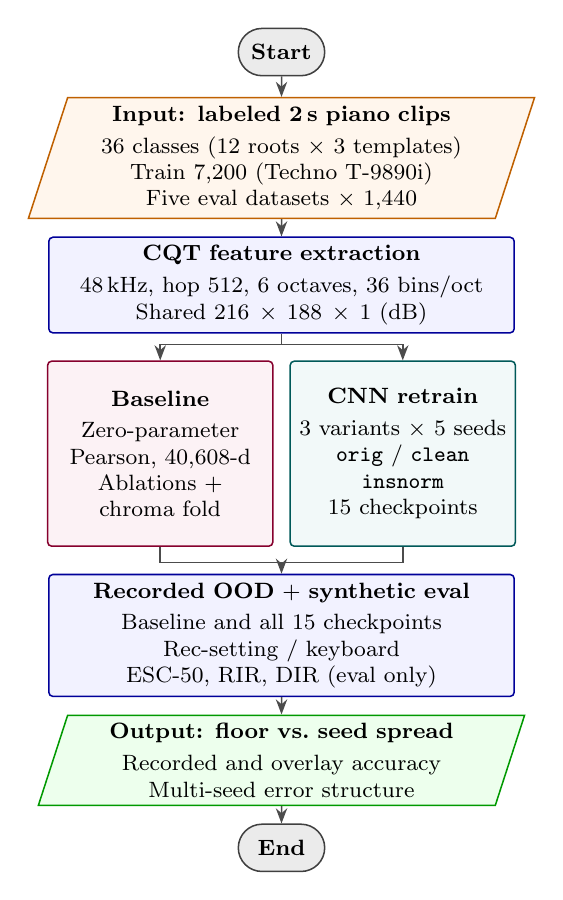
\begin{tikzpicture}[
    node distance=0.16cm and 0.10cm,
    >={Stealth},
    font=\footnotesize,
    base/.style={draw, align=center, minimum height=0.52cm, line width=0.55pt, inner sep=3pt},
    terminal/.style={base, shape=rounded rectangle, rounded rectangle arc length=180, draw=black!75, fill=black!8, minimum height=0.60cm, minimum width=1.8cm, inner xsep=10pt, inner ysep=2pt, font=\footnotesize\bfseries},
    process/.style={base, rectangle, rounded corners=1.5pt, draw=blue!60!black, fill=blue!5, text width=5.7cm},
    baseline/.style={base, rectangle, rounded corners=1.5pt, draw=purple!70!black, fill=purple!5, text width=2.65cm, minimum height=2.35cm},
    cnn/.style={base, rectangle, rounded corners=1.5pt, draw=teal!70!black, fill=teal!5, text width=2.65cm, minimum height=2.35cm},
    io/.style={base, trapezium, trapezium left angle=72, trapezium right angle=108, trapezium stretches body=true, draw=orange!75!black, fill=orange!7, text width=5.15cm, inner xsep=4pt},
    result/.style={base, trapezium, trapezium left angle=72, trapezium right angle=108, trapezium stretches body=true, draw=green!60!black, fill=green!7, text width=5.15cm, inner xsep=4pt},
    arrow/.style={->, line width=0.55pt, black!70}
  ]
    \node[terminal] (start) {Start};
    \node[io, below=0.26cm of start] (in1)
    {\textbf{Input: labeled 2\,s piano clips}\\[2pt]
     36 classes (12 roots $\times$ 3 templates)\\
     Train 7{,}200 (Techno T-9890i)\\
     Five eval datasets $\times$ 1{,}440};
    \node[process, below=0.22cm of in1] (p2)
    {\textbf{CQT feature extraction}\\[2pt]
     48\,kHz, hop 512, 6 octaves, 36 bins/oct\\
     Shared $216 \times 188 \times 1$ (dB)};
    \node[baseline, below left=0.34cm and 0.10cm of p2.south, anchor=north east] (base1)
    {\textbf{Baseline}\\[2pt]
     Zero-parameter\\
     Pearson, 40{,}608-d\\
     Ablations $+$ chroma fold};
    \node[cnn, below right=0.34cm and 0.10cm of p2.south, anchor=north west] (cnn1)
    {\textbf{CNN retrain}\\[2pt]
     3 variants $\times$ 5 seeds\\
     \texttt{orig} / \texttt{clean}\\
     \texttt{insnorm}\\
     15 checkpoints};
    \node[process, below=0.34cm of $(base1.south)!0.5!(cnn1.south)$, anchor=north] (p5)
    {\textbf{Recorded OOD $+$ synthetic eval}\\[2pt]
     Baseline and all 15 checkpoints\\
     Rec-setting / keyboard\\
     ESC-50, RIR, DIR (eval only)};
    \node[result, below=0.22cm of p5] (out)
    {\textbf{Output: floor vs.\ seed spread}\\[2pt]
     Recorded and overlay accuracy\\
     Multi-seed error structure};
    \node[terminal, below=0.22cm of out] (endn) {End};
    \draw[arrow] (start) -- (in1);
    \draw[arrow] (in1) -- (p2);
    \draw[arrow] (p2.south) -- ++(0,-0.14) -| (base1.north);
    \draw[arrow] (p2.south) -- ++(0,-0.14) -| (cnn1.north);
    \coordinate (merge) at ($(p5.north)+(0,0.14)$);
    \draw[line width=0.55pt, black!70] (base1.south) |- (merge);
    \draw[line width=0.55pt, black!70] (cnn1.south) |- (merge);
    \draw[arrow] (merge) -- (p5.north);
    \draw[arrow] (p5) -- (out);
    \draw[arrow] (out) -- (endn);
  \end{tikzpicture}%
  }
  \caption{Experimental pipeline. Shared CQT features feed a deterministic correlation baseline and a 15-checkpoint CNN retrain (3 variants $\times$ 5 seeds). Every classifier is scored on every recorded and synthetic condition. Overlays hit evaluation datasets only; CNN weights stay frozen.}
  \label{fig:methodology}
\end{figure}

\subsection{Two evaluation scenarios}\label{subsec3_0}

Scenario~1 (in-domain) holds instrument, room, and recording setting fixed and asks whether the CQT space separates the 36 classes at all. Five-fold cross-validation on the 7{,}200 Techno takes measures this; Section~\ref{subsec4_2} shows it is not the upper bound the phrase suggests.

Scenario~2 changes one factor at a time and tests each trained CNN checkpoint with no fine-tuning. Three recording-setting-shift datasets keep the Techno T-9890i and change the recording setup -- microphone, placement, and on-device signal chain, not the transducer alone (ThinkPad P14s Gen 2 Intel internal mic, Vivo Y27s phone, ASUS ROG Flow X13 2022 internal mic). Two keyboard-shift datasets then swap the instrument to a Yamaha PSR-S910 while reusing the ThinkPad and Flow recording setups already measured on the Techno. That pairing is the point: \texttt{thinkpad} versus \texttt{thinkpad-2} differs by keyboard, not by recording setup; \texttt{flow} versus \texttt{flow-2} does the same. \texttt{vivo} has no Yamaha counterpart, so it contributes recording-setting-shift evidence but not a matched pair. Table~\ref{tab:scenarios} lists every dataset. Synthetic overlays (Section~\ref{subsec3_7}) hit all five 1{,}440-sample datasets. No checkpoint is fine-tuned on evaluation data; the CNN's own retrain protocol (Section~\ref{subsec3_variants}) is a separate axis, not fine-tuning.

\begin{table*}[t]
\caption{Recorded evaluation datasets. The CNN is trained on \texttt{training} and evaluated on every dataset. $^\dagger$\texttt{vivo} has no Yamaha counterpart, so it does not enter the matched-pair analysis (Section~\ref{subsec4_3}).}\label{tab:scenarios}
\begin{tabular*}{\textwidth}{@{\extracolsep{\fill}}lllll@{}}
\toprule
Dataset & $N$ & Primary shift & Instrument & Recording setting \\
\midrule
\texttt{training} & 7{,}200 & None (in-domain) & Techno T-9890i & Xiaomi Redmi Pad 2 \\
\texttt{thinkpad} & 1{,}440 & Recording setting & Techno T-9890i & ThinkPad P14s Gen 2 (Intel) \\
\texttt{vivo} & 1{,}440 & Recording setting$^\dagger$ & Techno T-9890i & Vivo Y27s \\
\texttt{flow} & 1{,}440 & Recording setting & Techno T-9890i & ASUS ROG Flow X13 (2022) \\
\texttt{thinkpad-2} & 1{,}440 & Keyboard & Yamaha PSR-S910 & ThinkPad P14s Gen 2 (Intel) \\
\texttt{flow-2} & 1{,}440 & Keyboard & Yamaha PSR-S910 & ASUS ROG Flow X13 (2022) \\
\bottomrule
\end{tabular*}
\end{table*}

\subsection{Dataset acquisition}\label{subsec3_1}

A web recorder sends simultaneous MIDI note-on events over USB and captures the microphone. That removes manual playing errors and keeps the instrument's physical resonance and synthesis. The same trigger list and voicing are used for every dataset, so class identity does not change with the acoustic condition.

The vocabulary is 36 classes. Each class is a three-note piano sound: one of 12 roots (C, C$\sharp$, \ldots, B) times one of three interval templates (maj $+4,+3$; min $+3,+4$; dim $+3,+3$ semitones). A semitone is one chromatic step and occupies three CQT bins. Figures write \emph{C maj}, \emph{E dim}; file names keep the fourth-octave suffix. All takes sit in that octave, inside C1--C7 ($\approx$33--2093\,Hz) \cite{Telila2023}\cite{Harte2010}. The dim template places its three notes closer together than maj or min \cite{Byambatsogt2020}. Both instruments use a grand-piano preset; they still differ in sample set, loudspeaker, and cabinet.

\begin{enumerate}[1.]
\item \textbf{Training (\texttt{training})}: 200 samples per class, 7{,}200 total. Xiaomi Redmi Pad 2 mic, Techno T-9890i Acoustic Grand Piano. Attack delays 0--150\,ms approximate keystroke asynchrony \cite{Bella2011}. OGG/OPUS, 48{,}000\,Hz, 32-bit, mono, no filters. Sixteen clips (8\% of $C$ diminished, a recorder fault) are digital silence; Section~\ref{subsec3_variants} reports the CNN with and without them.
\item \textbf{Recording-setting shift (\texttt{thinkpad}, \texttt{vivo}, \texttt{flow})}: 40 per class, 1{,}440 each, WAV. Techno T-9890i on the ThinkPad P14s Gen 2 (Intel) internal mic, a Vivo Y27s phone mic, and the ASUS ROG Flow X13 (2022) internal mic.
\item \textbf{Keyboard shift (\texttt{thinkpad-2}, \texttt{flow-2})}: 40 per class, 1{,}440 each, WAV. Yamaha PSR-S910 on the ThinkPad and Flow recording setups already used on the Techno.
\end{enumerate}

No evaluation clip enters training, validation, early stopping, or hyperparameter choice.

\subsection{CQT feature extraction}\label{subsec3_2}

We compute CQT with \texttt{librosa.cqt()}. Each bin $f_k$ has constant quality
\begin{equation}
Q = \frac{f_k}{f_{k+1} - f_k} = \frac{1}{2^{1/B} - 1}
\label{eq:cqt}
\end{equation}
where $B$ is bins per octave \cite{Li2021}\cite{Lacoste2007}. Logarithmic spacing lines bins up with semitones, so a transposition is a vertical shift and a major third is the same bin distance on every root \cite{Harte2010}.

Table~\ref{tab:cqt-extraction-params} lists parameters. Thirty-six bins per octave (3 per semitone) resolve major ($+4,+3$), minor ($+3,+4$), and diminished ($+3,+3$) intervals \cite{Akram2025}\cite{OHanlon2021}. Each clip is truncated to a fixed 2.0\,s. Equation~\ref{eq:frames} gives 188 frames and a uniform shape $216 \times 188 \times 1$. Magnitudes go to dB with \texttt{librosa.amplitude\_to\_db(..., ref=np.max)} -- a per-clip reference that pins each clip's own loudest bin to 0\,dB before anything else in the pipeline runs. Because the dB floor (\texttt{top\_db}, 80\,dB below that same per-clip peak) is computed the same way regardless of the reference constant, changing \texttt{ref} only adds a uniform additive constant to a clip's dB values; the baseline classifier's own mean-centering (Section~\ref{subsec3_baseline}) is exactly invariant to that constant, so \texttt{ref=np.max} cannot be the source of any per-clip invariance measured later in this paper. The same parameters are used for training, every recorded dataset, and every overlay.

\begin{equation}
\text{frames} = \frac{\text{duration} \times \text{sample rate}}{\text{hop size}}
\label{eq:frames}
\end{equation}

\begin{table}[t]
\caption{CQT feature extraction parameters}\label{tab:cqt-extraction-params}
\begin{tabular}{@{}ll@{}}
\toprule
Parameter & Value \\
\midrule
Sample rate & 48{,}000\,Hz \\
Hop size & 512 samples \\
Octaves & 6 \\
Bins per octave & 36 \\
Total bins & 216 \\
Frequency range & C1 (32.70\,Hz) to C7 (2{,}093\,Hz) \\
Window & Hann \\
Frame length & 188 \\
Output shape & $216 \times 188 \times 1$ \\
\bottomrule
\end{tabular}
\end{table}

\begin{figure}[t]
\centering
\includegraphics[width=\columnwidth]{fig-cqt-train.png}
\caption{Training CQT of C maj ($+4,+3$) and C min ($+3,+4$): same root, one-semitone gap in the middle note. Frequency in Hz.}
\label{fig:cqt-spectrograms}
\end{figure}

\subsection{CNN architecture and training}\label{subsec3_3}

The CNN follows Wolf-Monheim \cite{Wolf-Monheim2025}, originally designed for environmental sound classification on ESC-50. Its compact four-block convolutional structure without recurrent layers or attention is appropriate for fixed-window classification from static spectrograms.

Table~\ref{tab:cnn-architecture} lists layers. Input batch normalization fits its scale and shift to the training distribution once and applies that fixed transform to every clip at inference (Section~\ref{sec1}); Section~\ref{subsec3_variants} replaces it with a per-clip alternative in one variant. The four Conv2D--MaxPooling2D blocks build a progressive hierarchy: the first block (64 filters) captures low-level spectral texture; the second (128 filters) encodes mid-level harmonic interval patterns; the third and fourth (256 filters each) represent chord-quality abstractions. The $3\times3$ receptive field matches the 1--2 bin frequency shifts that distinguish chord types, while MaxPooling provides spatial subsampling and limited translation invariance \cite{Purwono2022}. Dropout (rate 0.5) limits co-adaptation to the Techno piano voice.

\begin{table}[t]
\caption{CNN architecture specification}\label{tab:cnn-architecture}
\begin{tabularx}{\columnwidth}{@{}lXl@{}}
\toprule
Layer & Output shape & Notes \\
\midrule
BatchNorm & $216{\times}188{\times}1$ & Input normalization \\
Conv2D & $216{\times}188{\times}64$ & $3{\times}3$, ReLU, same \\
MaxPool & $108{\times}94{\times}64$ & $2{\times}2$, stride 2 \\
Conv2D & $108{\times}94{\times}128$ & $3{\times}3$, ReLU, same \\
MaxPool & $54{\times}47{\times}128$ & $2{\times}2$, stride 2 \\
Conv2D & $54{\times}47{\times}256$ & $3{\times}3$, ReLU, same \\
MaxPool & $27{\times}23{\times}256$ & $2{\times}2$, stride 2 \\
Conv2D & $27{\times}23{\times}256$ & $3{\times}3$, ReLU, same \\
MaxPool & $13{\times}11{\times}256$ & $2{\times}2$, stride 2 \\
Flatten & 36{,}608 & \\
Dense & 256 & ReLU \\
Dropout & 256 & rate 0.5 \\
Dense & 36 & Softmax \\
\bottomrule
\end{tabularx}
\end{table}

Training follows Table~\ref{tab:cnn-training-config}. Stratified 80/10/10 sampling keeps class balance, with the seed reused for the split, the weight initialization, and TensorFlow's global RNG. \texttt{ReduceLROnPlateau} multiplies the learning rate by 0.1 after 2 stagnant val-loss epochs; \texttt{EarlyStopping} stops after 6; max 50 epochs \cite{Wolf-Monheim2025}. The 10\% test split is held out of training and validation. This configuration is retrained 15 times, not once (Section~\ref{subsec3_variants}); Table~\ref{tab:cnn-training-config}'s seed value is the reference used for seed 42 of the retrain batch, not for every later test.

\begin{table}[t]
\caption{CNN training configuration}\label{tab:cnn-training-config}
\begin{tabular}{@{}ll@{}}
\toprule
Parameter & Value \\
\midrule
Reference seed & 42 \\
Train / Val / Test split & 80\% / 10\% / 10\% \\
Batch size & 32 \\
Initial learning rate & 0.001 \\
Optimizer & Adam \\
Weight initialization & Glorot uniform \\
Loss & Categorical cross-entropy \\
Max epochs & 50 \\
EarlyStopping patience & 6 epochs \\
ReduceLROnPlateau & factor 0.1, patience 2 \\
\bottomrule
\end{tabular}
\end{table}

\subsection{5-fold cross-validation}\label{subsec3_5}

Five folds on all 7{,}200 training samples, 80/20 per fold, measure in-domain score independent of one train/test split. Each fold retrains the CNN from a fresh random initialization and a fixed per-fold seed. Fold test partitions never enter training or early stopping for that fold.

\subsection{Correlation-centroid baseline}\label{subsec3_baseline}

A zero-parameter classifier is scored on the identical CQT features as a deterministic floor. Each class centroid is the mean of its flattened training CQT matrices ($216\times188 \to D=40{,}608$). A test clip is compared to all 36 centroids by Pearson correlation (both mean-centered and unit-normalized, then cosine similarity), so a uniform per-clip gain or offset in dB does not change the ranking. The classifier needs no gradient step, validation split, or seed. Section~\ref{subsec4_1} ablates the centering and scaling steps separately, scores the same features folded to a 12-bin chroma template, and scores the same centroids under the synthetic overlays.

\subsection{Measuring the envelope shift}\label{subsec3_drift}

The mechanism argument above -- that a uniform per-clip shift is what mean-centering removes -- is testable directly rather than only inferred from accuracy. For each class $k$, let $\bar x^{\text{train}}_k \in \mathbb{R}^D$ be the flattened-dB training centroid (mean over the 7{,}184 non-silent training clips of that class) and $\bar x^{\text{pack}}_k$ the same centroid computed on a held-out dataset's true-labeled clips. The drift is $\delta_k = \bar x^{\text{pack}}_k - \bar x^{\text{train}}_k$, decomposed into three mutually orthogonal parts:
\begin{align}
\delta_k^{\text{off}} &= (\delta_k^\top u)\,u, \qquad u = \mathbf{1}/\sqrt{D} \label{eq:off}\\
\delta_k^{\text{sc}} &= \big((\delta_k - \delta_k^{\text{off}})^\top t_k\big)\,t_k \label{eq:sc}\\
\delta_k^{\text{res}} &= \delta_k - \delta_k^{\text{off}} - \delta_k^{\text{sc}} \label{eq:res}
\end{align}
where $t_k = (\bar x^{\text{train}}_k - \overline{\bar x^{\text{train}}_k}) / \lVert \bar x^{\text{train}}_k - \overline{\bar x^{\text{train}}_k} \rVert$ is that class's own training centroid, mean-centered and unit-normalized. $\delta_k^{\text{off}}$ is the drift's projection onto the all-ones direction: a uniform per-clip dB level shift, exactly what mean-centering removes. $\delta_k^{\text{sc}}$ is the remainder's projection onto $t_k$: a contrast or gain change on that class's own harmonic pattern, what unit-normalizing additionally removes. Because $t_k$ is mean-centered, $u \perp t_k$, so all three components are mutually orthogonal and
\begin{equation}
\lVert\delta_k\rVert^2 = \lVert\delta_k^{\text{off}}\rVert^2 + \lVert\delta_k^{\text{sc}}\rVert^2 + \lVert\delta_k^{\text{res}}\rVert^2,
\label{eq:pythagoras}
\end{equation}
so the three energy shares ($\lVert\cdot\rVert^2/\lVert\delta_k\rVert^2$) sum to exactly 1. That identity is what makes "percent of drift explained" well defined here rather than an arbitrary choice of norm. Section~\ref{subsec4_1} reports $1 - \lVert\delta_k^{\text{res}}\rVert^2/\lVert\delta_k\rVert^2$, averaged over the 36 classes, per held-out dataset.

\subsection{CNN retrain variants and multi-seed protocol}\label{subsec3_variants}

Three points in the training design are varied against Section~\ref{subsec3_3}'s architecture. \texttt{orig} matches Table~\ref{tab:cnn-training-config} exactly, including the sixteen silent clips (7{,}200 clips). \texttt{clean} drops them (7{,}184 clips). \texttt{insnorm} replaces input \texttt{BatchNormalization} with per-sample standardization, $x' = (x-\mu_x)/(\sigma_x+\epsilon)$ computed independently per clip rather than fit once over training and applied identically at inference; \texttt{insnorm} always trains on the same cleaned 7{,}184-clip set as \texttt{clean} -- it is not a fourth, silence-kept configuration, so it isolates the normalization change only relative to \texttt{clean}, and the \texttt{orig}-versus-\texttt{clean} columns in Table~\ref{tab:cross-domain} are what isolates the silence fix on its own. Each variant is retrained from five seeds (42--46); Section~\ref{subsec4_3} pools accuracy across the five per variant on the recorded datasets, and Section~\ref{subsec4_4} does the same under synthetic overlays. One further control (Section~\ref{subsec4_5}) retrains \texttt{insnorm}/seed 43 with $\epsilon$ raised a thousand-fold, everything else unchanged, to test whether its collapse (below) is numerical or architectural.

\subsection{Synthetic overlays: environment and a second recording-setting axis}\label{subsec3_7}

Three overlays hit already out-of-domain datasets without retraining, applied to all fifteen CNN checkpoints and to the baseline. Two proxy environment shift, the factor with no recorded dataset in this design: ESC-50 interior noise and indoor room impulse responses. The third, microphone impulse response, proxies a second, independent axis of recording-setting shift alongside the three recorded microphone changes -- a synthetic transducer swap layered on an already recorded consumer microphone. Overlay probability is 1 (every evaluation sample is degraded), the draw is random per sample with a fixed seed, and wet waveforms are not written back into the training tree. The same five datasets are used for all three overlays, so deltas are comparable.

\textbf{Additive noise.} ESC-50 interior/domestic clips \cite{Piczak2015} are converted to CQT with the same hop and binning as the chord features, yielding a 400-clip bank over 10 classes. Mixing is performed in the CQT power domain at a uniform SNR drawn from $[10, 25]$\,dB (realized mean 17.5\,dB) with a random time roll. This is a controlled interior overlay, not a claim that ESC-50 matches any one room.

\textbf{Room impulse responses.} Indoor IRs from the McDermott IR Survey \cite{Traer2016} are resampled to 48\,kHz and trimmed of leading silence. Bathrooms, showers, and outdoor/transit rooms are excluded, leaving 174 indoor IRs. Each evaluation waveform is convolved with a randomly drawn IR, cropped, peak-normalized, and converted to CQT.

\textbf{Device impulse responses.} Six measured microphone IRs (AKG D12, Crystal, Lomo 52A-5M, Melodium RM6, Oktava MD57, STC 4035) are preprocessed identically and convolved one-per-sample onto the same five datasets. They probe a second, synthetic recording-setting axis: microphone frequency response in isolation, layered on the placement and signal-chain differences already present in the three recorded recording-setting datasets.

These overlays test a clean-trained CQT--CNN and the deterministic baseline alike. They are not a training recipe, and they are applied independently: a noise trial does not also convolve an IR, so noise, RIR, and DIR remain single-factor and are reported separately (Table~\ref{tab:aug}), not only pooled into the two shift factors they proxy.

\subsection{Evaluation metrics}\label{subsec3_6}

Accuracy, precision, recall, and F1 come from the confusion matrix. For a one-versus-rest partition of a single class the counts are True Positives (TP), True Negatives (TN), False Positives (FP), and False Negatives (FN):
\begin{equation}
\mathrm{P}=\frac{\mathrm{TP}}{\mathrm{TP}+\mathrm{FP}},\quad
\mathrm{R}=\frac{\mathrm{TP}}{\mathrm{TP}+\mathrm{FN}},\quad
\mathrm{F1}=\frac{2\mathrm{PR}}{\mathrm{P}+\mathrm{R}}.
\label{eq:prf}
\end{equation}
Accuracy is the fraction of clips with the correct label. Macro P, R, and F1 are unweighted means over the 36 classes. Per-class recall, pooled over the 5-seed retrain batch, shows which classes collapse and how consistently (Section~\ref{subsec4_3}).

\section{Results}\label{sec4}

\subsection{Baseline versus the CNN: what is actually doing the work}\label{subsec4_1}

Table~\ref{tab:cross-domain} and Fig.~\ref{fig:cross-domain} compare the deterministic correlation-centroid baseline (Section~\ref{subsec3_baseline}) against the CNN's three retrain variants, pooled across 5 seeds each. The baseline reaches 1.000 on every held-out recording, recording-setting shift and keyboard shift alike. \texttt{insnorm} is reported two ways: excluding one seed that collapsed during training (n=4, the generalization-comparable reading) and including it (n=5, the honest reading of what five independent retrains actually produced) -- both are in Table~\ref{tab:cross-domain} rather than only the favorable exclusion. On the excluded reading, the baseline still out-performs every CNN variant on every dataset, by 2--19 points; on the included reading, the collapsed seed alone drags \texttt{insnorm}'s mean below \texttt{orig} on four of five datasets, which is why Section~\ref{subsec4_5} treats that collapse as a real finding, not an outlier to discard.

Is the baseline's ceiling automatic? Three checks say no. First, an ablation of its own two operations: scoring the same centroids by raw Euclidean distance (neither centered nor scaled) falls to 0.859--1.000; scaling only (dividing by each vector's own standard deviation, no mean removal) falls to 0.988--0.999; centering only (mean removal, Euclidean distance, no rescaling) reaches 1.000 on every dataset, matching full correlation; cosine similarity with scaling but no centering reaches 0.998--1.000. Centering alone is nearly sufficient and scaling alone is close; only using neither breaks. Second, a coarser standard-MIR representation: folding the same 216 CQT bins to a 12-bin chroma/PCP template (Section~\ref{subsec4_1}'s classifier unchanged, only the input aggregated) reaches 0.98--1.00 in the dB domain but only 0.42--0.93 in the power domain -- collapsing the representation is not free, and the log compression the CQT pipeline already applies is itself doing real work, not just the per-clip centering. Third, a margin check: because the baseline needs only that the true class rank first among 36, not that drift vanish, per-clip cosine margins (true-class similarity minus the best wrong class) are strictly positive everywhere tested -- minimum 0.024--0.050, median 0.098--0.122 across the five datasets -- which is why Section~\ref{subsec3_drift}'s 30--56\% drift explained by offset and scale (mean 44\%, Section~\ref{subsec5_0}) is enough for 1.000 accuracy without being close to 100\%.

\begin{table}[htbp]
\caption{Out-of-domain accuracy: deterministic baseline vs.\ CNN variant means over 5 seeds each. \texttt{insnorm} is reported both ways: n=4 excludes its one training-collapse seed (Section~\ref{subsec4_5}); n=5 includes it. sd in text (Section~\ref{subsec5_0}).}\label{tab:cross-domain}
\setlength{\tabcolsep}{3pt}
\begin{tabular}{@{}lrrrrr@{}}
\toprule
Dataset & Baseline & \texttt{orig} & \texttt{clean} & \texttt{insnorm}$_{n4}$ & \texttt{insnorm}$_{n5}$ \\
\midrule
\texttt{thinkpad} & 1.000 & 0.961 & 0.962 & 0.976 & 0.786 \\
\texttt{vivo} & 1.000 & 0.903 & 0.894 & 0.989 & 0.797 \\
\texttt{flow} & 1.000 & 0.911 & 0.900 & 0.993 & 0.800 \\
\texttt{thinkpad-2} & 1.000 & 0.803 & 0.719 & 0.908 & 0.732 \\
\texttt{flow-2} & 1.000 & 0.815 & 0.728 & 0.917 & 0.739 \\
\bottomrule
\end{tabular}
\end{table}

\begin{figure}[htbp]
\centering
\includegraphics[width=\columnwidth,height=0.26\textheight,keepaspectratio]{fig-cross-domain.pdf}
\caption{Out-of-domain accuracy: deterministic baseline vs.\ CNN variants, mean $\pm$ sd over seeds (\texttt{insnorm}'s collapsed seed excluded; Section~\ref{subsec4_1}).}
\label{fig:cross-domain}
\end{figure}

Any single seed's number sits inside, not at the edge of, a spread the full retrain batch shows is wide: on \texttt{thinkpad-2}, \texttt{orig} ranges 0.705--0.963 across its five seeds and \texttt{clean} ranges 0.348--0.925, at fixed in-domain accuracy of 1.00 for all of them. A domain-shift cost expressed as one seed's number is, by this evidence, mostly reporting where that seed's optimizer landed.

\subsection{In-domain accuracy is not an upper bound}\label{subsec4_2}

Under Scenario~1 the CNN scores 1.00 accuracy, precision, recall, and F1 on every fold of the 7{,}200 Techno takes, and on the held-out test split of every one of the fifteen retrains ($1.000\pm0.000$ for \texttt{orig} and \texttt{insnorm}, $0.9997\pm0.0006$ for \texttt{clean}) -- which certifies only that the classes are separable, not that a trained instance generalizes: Section~\ref{subsec4_1} shows the same fifteen models spread from 0.35 to 1.00 accuracy on held-out recordings. The baseline makes the same point more starkly in the opposite direction. Its own 5-fold in-domain accuracy is $0.9974\pm0.0007$ (all 7{,}200 training clips) or $0.9996\pm0.0006$ (the 7{,}184 non-silent clips) -- both \emph{below} its 1.000 on every held-out dataset. The five held-out datasets, one MIDI-triggered voicing each, are not an easier oracle case than the training pool's own held-out fold; "in-domain" and "easy" are not the same property.

\subsection{Multi-seed error structure}\label{subsec4_3}

A single retrained checkpoint's error list does not predict another seed's. On \texttt{thinkpad-2}, \texttt{orig}/seed 42 has exactly one zero-recall class ($D$ diminished); seed 43 has five ($A$ diminished, $B$ major, $D$ diminished, $D$ minor, $G\sharp$ diminished); seed 44 has two ($A$ diminished, $D$ diminished); seed 45 has five again, but a different five ($A\sharp$ diminished, $A$ diminished, $A$ major, $D$ major, $F\sharp$ minor); seed 46 has two, different again ($C\sharp$ major, $F$ diminished). Reporting any one seed's confusion matrix as \emph{the} CNN's error structure, as though it generalized to the architecture rather than to that specific trained instance, repeats the single-run problem Section~\ref{subsec4_2} raises for accuracy, one level down.

Fig.~\ref{fig:perclass} pools zero-recall fraction across all five seeds per variant on both keyboard-shift datasets (\texttt{insnorm}'s collapsed seed excluded, since it zeroes every class and carries no per-class information). $E$ diminished has zero recall in \emph{none} of the fifteen retrains' seeds, on either dataset, under any variant, despite showing up in individual seeds' confusion matrices as an occasional failure. $D$ minor and $G\sharp$ diminished each go to zero in 1 of 5 seeds under \texttt{orig} and \texttt{clean} on both datasets -- present, but not the dominant pattern. The classes that come closest to a stable collapse are $A$ diminished and $D$ diminished: under \texttt{clean}, $A$ diminished has zero recall in 4 of 5 seeds on \texttt{thinkpad-2} and 3 of 5 on \texttt{flow-2}, the only two classes that reach $\geq$2 zero-recall seeds on \emph{both} Yamaha datasets for any variant. \texttt{insnorm}, at 4 surviving seeds, has no class that repeats even once. The honest claim is not a fixed list of failure classes; it is that some class collapses on a given retrain, which class is mostly seed-specific, and \texttt{insnorm} is the only variant tested here without a repeat offender.

\begin{figure*}[t]
\centering
\includegraphics[width=0.85\textwidth,keepaspectratio]{fig-perclass-multiseed.pdf}
\caption{Fraction of the 5-seed retrain batch with zero recall, per class, on both keyboard-shift datasets (\texttt{insnorm}'s collapsed seed excluded). Classes with zero recall in no seed of any variant are omitted.}
\label{fig:perclass}
\end{figure*}

\subsection{Synthetic overlays: environment and recording-setting shift}\label{subsec4_4}

Table~\ref{tab:aug} and Fig.~\ref{fig:aug} score the deterministic baseline and the CNN's three variants under each of the three synthetic overlays separately, pooled across the same 5 seeds as Section~\ref{subsec4_1} (\texttt{insnorm}'s collapsed seed excluded). The baseline is unaffected: 0.9997--1.000 under every overlay, matching its 1.000 on the five recorded datasets. Every CNN variant is worse under noise than under RIR, and worse under RIR than under the recording-setting overlay (DIR): \texttt{orig} 0.770 / 0.817 / 0.879, \texttt{clean} 0.750 / 0.779 / 0.824, \texttt{insnorm} 0.913 / 0.935 / 0.966. \texttt{insnorm} again has the highest mean and roughly half the seed variance of \texttt{orig}/\texttt{clean} on every overlay, and its own noise-to-DIR gap (5.3 points) is smaller than \texttt{orig}'s (10.9 points) or \texttt{clean}'s (7.4 points): per-sample standardization narrows, without closing, both the baseline gap and this asymmetry. DIR is not uniformly a tax -- it raises accuracy on some datasets and lowers it on others, and pooling it with RIR into a single "recording setting" number would have hidden that (Section~\ref{subsec5_2}).

Per dataset, \texttt{orig}'s noise tax (recorded accuracy minus noise accuracy, Table~\ref{tab:cross-domain} vs.\ this table) is 6.5--10.3 points on the three recording-setting-shift datasets and 14.5--15.3 points on the two keyboard-shift datasets: environment shift compounds keyboard shift rather than substituting for it. Scoring the baseline's centroids by raw Euclidean distance under the same overlays reproduces the same ordering and is worse than the recorded-shift ablation: mean accuracy falls to 0.749 under noise, 0.921 under RIR, 0.937 under DIR. Per-clip mean-centering and unit-normalization is what keeps the correlation classifier at 1.000 under every condition tested here, recorded or synthetic; without it, environment shift is the hardest condition in the entire dataset.

\begin{table}[htbp]
\caption{Accuracy under synthetic overlays, pooled over 5 seeds (4 for \texttt{insnorm}, collapsed seed excluded), by overlay type rather than pooled factor.}\label{tab:aug}
\begin{tabular}{@{}lrrrr@{}}
\toprule
Overlay & Baseline & \texttt{orig} & \texttt{clean} & \texttt{insnorm} \\
\midrule
Noise & 1.000 & 0.770 & 0.750 & 0.913 \\
RIR & 1.000 & 0.817 & 0.779 & 0.935 \\
DIR & 1.000 & 0.879 & 0.824 & 0.966 \\
\bottomrule
\end{tabular}
\end{table}

\begin{figure}[htbp]
\centering
\includegraphics[width=\columnwidth,height=0.26\textheight,keepaspectratio]{fig-aug-compare.pdf}
\caption{Accuracy under each synthetic overlay, pooled over 5 seeds: deterministic baseline vs.\ CNN variants (\texttt{insnorm}'s collapsed seed excluded; Section~\ref{subsec4_4}).}
\label{fig:aug}
\end{figure}

\subsection{Does the \texttt{insnorm} collapse have a numerical fix?}\label{subsec4_5}

One seed (43) of the \texttt{insnorm} retrain batch collapsed to exact chance accuracy (0.0278, $=1/36$) from epoch 1, with training loss stuck at $\ln 36 \approx 3.58$, and reproduced identically on retrain -- a deterministic instability. The stated mechanism is that per-sample standardization has no learnable scale or shift to recover from a bad initialization, unlike \texttt{BatchNormalization}'s learned $\gamma,\beta$. That claim is falsifiable: if the collapse were instead a numerical artifact of the layer's stability constant $\epsilon=10^{-6}$, raising $\epsilon$ should fix it without touching the architecture. Retraining the identical (\texttt{insnorm}, seed 43) configuration with $\epsilon=10^{-3}$, a thousand-fold increase, reproduces the collapse exactly: 7 epochs, final training loss 3.583, test accuracy 0.0278. The failure is architectural, not numerical, and a practical recommendation to use \texttt{insnorm} should assume this collapse recurs at some rate across seeds rather than treat it as a one-off.

\section{Discussion}\label{sec5}

\subsection{What the baseline explains}\label{subsec5_0}

A single seed's reading is not a safe stand-in for the keyboard-shift cost. \texttt{orig} spans 0.705--0.963 on \texttt{thinkpad-2} by seed alone (Section~\ref{subsec4_1}), wider than the gap between recording-setting shift and keyboard shift it would be used to measure. The shift is still real -- mean CNN accuracy is lower on both Yamaha datasets than on any recording-setting-shift dataset, for every variant -- but its \emph{size}, read from one seed, is mostly reporting where that seed's optimizer landed.

Two direct measurements explain why the baseline is largely immune to a shift the CNN finds expensive. Per-clip mean CQT level is $-51.9$\,dB in training and ranges $-60.3$\,dB (\texttt{vivo}) to $-44.7$\,dB (\texttt{thinkpad-2}) across the five recorded datasets -- a shift of exactly the kind mean-centering removes by construction. The offset-plus-scale decomposition (Section~\ref{subsec3_drift}) accounts for 30--56\% of each class centroid's drift (mean 44\%, five datasets); Section~\ref{subsec4_1}'s margin check shows that is enough for 1.000 accuracy without needing to be close to 100\%, since classification needs only that the true class outrank 35 others. The same operation reaches $\geq$0.9997 under every synthetic overlay tested (Section~\ref{subsec4_4}), recording-setting and environment alike, and holds up against a coarser chroma fold and against dropping either half of centering-and-scaling on its own (Section~\ref{subsec4_1}) -- this is not a single ablation's accident. The CNN's input \texttt{BatchNormalization} cannot do the equivalent: fit once on the training distribution, it applies one fixed affine transform to every clip at inference, centering the training distribution but not a shift specific to one held-out recording or overlay -- the exact failure mode covariate-shift-aware normalization work anticipates \cite{Li2016}\cite{Ulyanov2016}. \texttt{insnorm} raises the mean and roughly halves the seed variance on every condition tested, recorded and synthetic, without matching the baseline and without avoiding a training collapse a thousand-fold larger $\epsilon$ does not fix (Section~\ref{subsec4_5}) -- evidence for the mechanism, and evidence that a per-sample operation with no learnable recovery path is not a drop-in production fix.

None of this means the baseline is a chord-recognition system to deploy. Its 1.000 accuracy is a property of this protocol -- MIDI-triggered onsets, one fixed voicing, isolated 2\,s triads, a shared trigger list across every dataset -- not evidence that per-clip correlation matching would separate 36 chords played with expressive timing, dynamics, or a wider harmonic vocabulary. What it is evidence for is narrower and still useful: on this protocol, the measured domain-shift cost is largely a removable per-clip effect, not evidence that the classes overlap under shift, and a trained CNN's single-run number conflates the two.

\subsection{CNN error structure is mostly seed-specific}\label{subsec5_1}

Section~\ref{subsec4_3}'s multi-seed result changes what can be claimed about which classes fail and why. No fixed group of classes replicates across the fifteen retrained checkpoints; $E$ diminished, a class that shows up as a total failure in some individual seeds' confusion matrices, has zero recall in none of them once all fifteen are read together. What does hold up, weakly, is that \texttt{clean} produces a repeat offender ($A$ diminished, both Yamaha datasets, most seeds) that \texttt{orig} and \texttt{insnorm} do not. A shared-tone or harmonic-proximity account of \emph{why} a given seed's model confuses two specific chords -- close triads, one semitone apart, sharing a root and fifth -- is still consistent with individual confusion matrices, but it explains a property of one trained instance, not a property of the task or the acoustic shift. The instance-level account and the task-level account answer different questions, and Section~\ref{subsec4_2}'s in-domain result already rules out the task-level version: the classes are separable, every time, regardless of which classes a given retrain happens to confuse.

\subsection{Synthetic overlays: DIR is not a uniform tax}\label{subsec5_2}

Un-pooling the overlay results (Table~\ref{tab:aug}) shows two things a two-factor summary would hide. Additive noise is the most consistent harm across every variant and every dataset; RIR is smaller and still a net cost; DIR moves accuracy by less on average but not uniformly -- it lowers \texttt{orig}'s accuracy on \texttt{vivo} and \texttt{flow} and raises it elsewhere, a chance move of a specific spectrum toward the training envelope, not a pre-process to ship. A pooled "environment vs.\ recording setting" summary would be correct on average and wrong about DIR specifically.

Edwards et al.\ \cite{Edwards2024} applied test-time noise and reverb to a clean-trained transcription model and saw drops of several to about 19 note-onset F1 points on MAPS, then recovered the OOD set with train-time mixing -- a different protocol (train-time intervention) and a different task (onset transcription) from this paper's eval-only, chord-classification design. Our pooled noise tax, 6.5--15.3 accuracy points depending on the dataset, sits in a comparable range despite that difference, which is coincidental agreement in magnitude, not evidence the two studies measure the same thing. The nearer peer group for this paper's actual contribution is not augmentation-recovery work but the smaller literature on reproducibility and simple baselines under distribution shift \cite{Bouthillier2021}\cite{Geirhos2020} -- work asking whether a benchmark result reflects the property it claims to, which is the question Sections~\ref{subsec4_1}--\ref{subsec4_3} answer for this one.

\subsection{Limitations}\label{subsec5_3}

Both instruments are digital pianos on a grand-piano preset; an acoustic grand would be a larger keyboard factor. All voicings are isolated fourth-octave triads, and training uses one tablet microphone. \texttt{vivo} has no keyboard-shift counterpart, so it contributes to the recording-setting-shift pool (Tables~\ref{tab:cross-domain}, \ref{tab:aug}) but not to the matched-pair error analysis. The training set's sixteen silent clips (Section~\ref{subsec3_variants}) went undetected by resubstitution accuracy; dropping them (\texttt{clean}) is not uniformly better than keeping them (\texttt{orig}) out-of-domain on any dataset -- a data-quality fix that looks obviously correct in-sample does not obviously generalize, which is itself worth flagging rather than treating as a footnote. \texttt{insnorm}'s collapsed seed is architectural, not fixed by a larger $\epsilon$ (Section~\ref{subsec4_5}); a learnable per-sample affine parameter, which would also resolve the broken \texttt{load\_model()} deserialization noted in the code release, is the natural next thing to try and was not trained this round. The drift decomposition's residual, 44--70\% of centroid drift depending on the dataset, is not attributed to a specific cause; it may include genuine musical or timbral variation the mean-and-scale model cannot separate from measurement noise. No recorded dataset covers environmental shift directly; the noise and RIR overlays are a controlled proxy, not a recorded room. The baseline has no mechanism for musical variation beyond this protocol's fixed voicing; it is a floor, not a proposed chord-recognition system.

\section{Conclusion}\label{sec6}

On this protocol, in-domain accuracy and a single OOD run are both misleading on their own. A zero-parameter correlation nearest-centroid classifier reaches 1.000 accuracy on every held-out recording and 0.999--1.000 under every synthetic overlay, higher than its own in-domain accuracy -- so the held-out datasets are not an easier case, and the ceiling survives an ablation of its own mechanism, a coarser chroma representation, and a rank-1 margin check. The CQT--CNN trained on the same features reaches 1.00 in-domain on every one of fifteen retrains, but which classes it fails on OOD is mostly seed-specific: no group of classes repeats across retrains, and a class that looks like a total failure in one seed's confusion matrix can have zero recall in none of the other fourteen. Per-sample standardization in place of batch normalization raises mean accuracy and roughly halves seed variance on every condition tested, recorded and synthetic, without closing the gap to the baseline and without escaping a training collapse that a thousand-fold larger stability constant does not fix -- an architectural cost, disclosed rather than hidden inside a favorable seed exclusion.

We withheld train-time mixing so the recorded numbers stay a factorized reading of a fixed CQT--CNN, now measured against a floor a template match already reaches under every recorded and synthetic condition here. The recommendation is not that this baseline should be deployed; it is that any future claim about this protocol's domain-shift cost -- CQT-based or not -- should be checked against a deterministic floor and a multi-seed spread before it is checked against nothing but in-domain 1.00 and one run.

\backmatter

\bmhead{Author contributions}
All authors contributed to study conceptualization and design. Material preparation, data acquisition, experimentation, analysis, and drafting were performed by CGS. All authors reviewed and approved the final version.

\bmhead{Funding}
No funding was received for this work.

\bmhead{Data availability}
The piano chord dataset is publicly available at \url{https://zenodo.org/records/21077144}.

\bmhead{Code availability}
The dataset generation and recording tool is available at \url{https://github.com/sglkc/chords-dataset-generator/}. Experiment notebooks are available in the project repository.

\section*{Declarations}

\bmhead{Conflict of interest}
The authors declare no competing interests.

\bmhead{Ethics approval}
Not applicable.

\bmhead{Consent for publication}
All authors approved the final manuscript.

\bibliography{mendeley}

\end{document}
